\begin{figure*}[t]
\centering
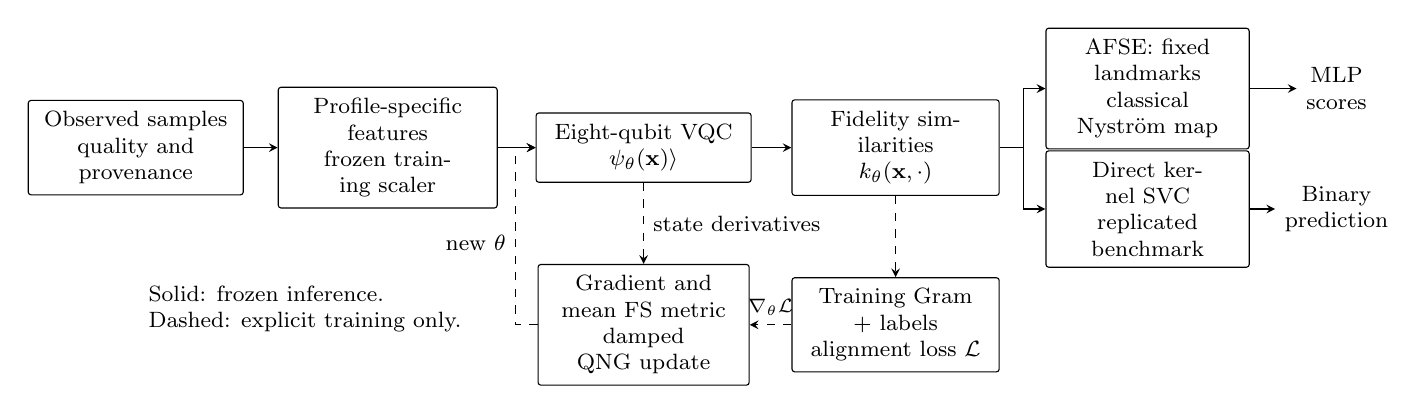
\begin{tikzpicture}[x=1cm,y=1cm,>=stealth,
  box/.style={draw,rounded corners=1pt,align=center,font=\footnotesize,inner sep=4pt,minimum height=0.82cm},
  small/.style={font=\footnotesize,align=center}]
\node[box,text width=2.45cm] (obs) at (0,0) {Observed samples\\quality and provenance};
\node[box,text width=2.50cm] (feat) at (3.20,0) {Profile-specific features\\frozen training scaler};
\node[box,text width=2.45cm] (state) at (6.45,0) {Eight-qubit VQC\\$\lvert\psi_{\boldsymbol\theta}(\mathbf x)\rangle$};
\node[box,text width=2.35cm] (kernel) at (9.65,0) {Fidelity similarities\\$k_{\boldsymbol\theta}(\mathbf x,\cdot)$};
\draw[->] (obs)--(feat); \draw[->] (feat)--(state); \draw[->] (state)--(kernel);
\node[box,text width=2.3cm] (afse) at (12.85,0.75) {AFSE: fixed landmarks\\classical Nystr\"om map};
\node[box,text width=2.3cm] (svm) at (12.85,-0.78) {Direct kernel SVC\\replicated benchmark};
\draw[->] (kernel.east) -- ++(0.30,0) |- (afse.west);
\draw[->] (kernel.east) -- ++(0.30,0) |- (svm.west);
\node[small] (mlp) at (15.25,0.75) {MLP\\scores};
\node[small] (binary) at (15.25,-0.78) {Binary\\prediction};
\draw[->] (afse.east)--(mlp.west); \draw[->] (svm.east)--(binary.west);
\node[box,text width=2.35cm] (loss) at (9.65,-2.25) {Training Gram + labels\\alignment loss $\mathcal L$};
\node[box,text width=2.4cm] (qng) at (6.45,-2.25) {Gradient and mean FS metric\\damped QNG update};
\draw[->,dashed] (kernel.south)--(loss.north);
\draw[->,dashed] (loss.west)-- node[above,font=\scriptsize] {$\nabla_{\boldsymbol\theta}\mathcal L$} (qng.east);
\draw[->,dashed] (state.south)-- node[right,font=\footnotesize] {state derivatives} (qng.north);
\draw[->,dashed] (qng.west)-- ++(-0.28,0) |- node[pos=0.23,left,font=\footnotesize] {new $\boldsymbol\theta$} (state.west);
\node[small,align=left] at (2.15,-2.05) {Solid: frozen inference.\\Dashed: explicit training only.};
\end{tikzpicture}
\caption{AQSE processing boundaries. The network demonstrator uses State8 and the AFSE--MLP branch. The 30-replica experiment uses harmonic features and the direct-kernel SVC branch. Labels enter the training objective, not the observed feature vector. The mean Fubini--Study (FS) metric is computed from state derivatives, separately from the loss gradient. No simulator truth enters inference.}
\label{fig:aqse-routes}
\end{figure*}
